


\tikzset{every picture/.style={line width=0.75pt}} %set default line width to 0.75pt

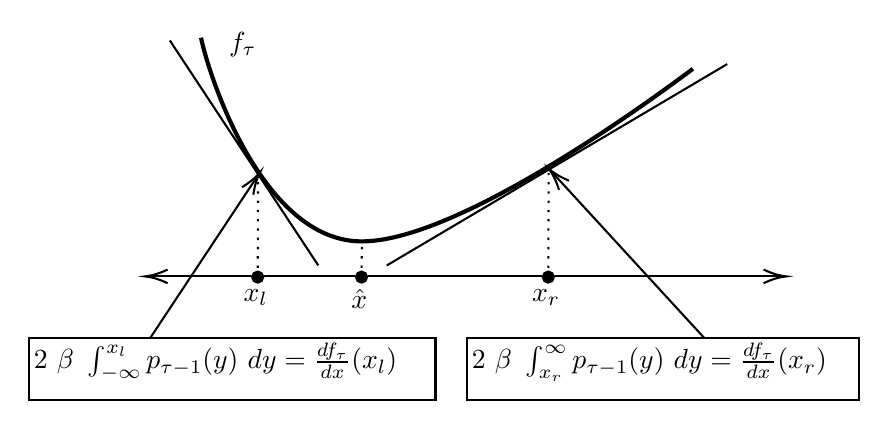
\begin{tikzpicture}[x=0.75pt,y=0.75pt,yscale=-1,xscale=1]
%uncomment if require: \path (0,308); %set diagram left start at 0, and has height of 308

%Curve Lines [id:da37061921880533877]
\draw [line width=1.5]    (98,85.33) .. controls (102.36,105.81) and (127.25,179.72) .. (172,183.33) .. controls (216.75,186.95) and (312.43,117.26) .. (335,100.33) ;
%Straight Lines [id:da8132100594867722]
\draw    (73,200.33) -- (378,200.33) ;
\draw [shift={(380,200.33)}, rotate = 180] [color={rgb, 255:red, 0; green, 0; blue, 0 }  ][line width=0.75]    (10.93,-3.29) .. controls (6.95,-1.4) and (3.31,-0.3) .. (0,0) .. controls (3.31,0.3) and (6.95,1.4) .. (10.93,3.29)   ;
\draw [shift={(71,200.33)}, rotate = 0] [color={rgb, 255:red, 0; green, 0; blue, 0 }  ][line width=0.75]    (10.93,-3.29) .. controls (6.95,-1.4) and (3.31,-0.3) .. (0,0) .. controls (3.31,0.3) and (6.95,1.4) .. (10.93,3.29)   ;
%Shape: Circle [id:dp2801837798690885]
\draw  [fill={rgb, 255:red, 0; green, 0; blue, 0 }  ,fill opacity=1 ] (172.67,200.67) .. controls (172.67,199.19) and (173.86,198) .. (175.33,198) .. controls (176.81,198) and (178,199.19) .. (178,200.67) .. controls (178,202.14) and (176.81,203.33) .. (175.33,203.33) .. controls (173.86,203.33) and (172.67,202.14) .. (172.67,200.67) -- cycle ;
%Shape: Circle [id:dp9237316574850754]
\draw  [fill={rgb, 255:red, 0; green, 0; blue, 0 }  ,fill opacity=1 ] (262.67,200.67) .. controls (262.67,199.19) and (263.86,198) .. (265.33,198) .. controls (266.81,198) and (268,199.19) .. (268,200.67) .. controls (268,202.14) and (266.81,203.33) .. (265.33,203.33) .. controls (263.86,203.33) and (262.67,202.14) .. (262.67,200.67) -- cycle ;
%Shape: Circle [id:dp045787056716331875]
\draw  [fill={rgb, 255:red, 0; green, 0; blue, 0 }  ,fill opacity=1 ] (122.67,200.67) .. controls (122.67,199.19) and (123.86,198) .. (125.33,198) .. controls (126.81,198) and (128,199.19) .. (128,200.67) .. controls (128,202.14) and (126.81,203.33) .. (125.33,203.33) .. controls (123.86,203.33) and (122.67,202.14) .. (122.67,200.67) -- cycle ;
%Straight Lines [id:da08221456294078888]
\draw    (83,86.67) -- (154.52,195.05) ;
%Straight Lines [id:da4107386957452337]
\draw    (351.52,98.05) -- (187.52,195.05) ;
%Straight Lines [id:da4276666085658716]
\draw  [dash pattern={on 0.84pt off 2.51pt}]  (125.33,200.67) -- (125.52,149.05) ;
%Straight Lines [id:da6234026284865279]
\draw  [dash pattern={on 0.84pt off 2.51pt}]  (265.33,200.67) -- (265.52,146.38) ;
%Straight Lines [id:da7796663876642187]
\draw  [dash pattern={on 0.84pt off 2.51pt}]  (175.33,200.67) -- (175.52,184.05) ;
%Straight Lines [id:da05642327969494221]
\draw    (73.52,230.05) -- (125.42,151.71) ;
\draw [shift={(126.52,150.05)}, rotate = 483.52] [color={rgb, 255:red, 0; green, 0; blue, 0 }  ][line width=0.75]    (10.93,-3.29) .. controls (6.95,-1.4) and (3.31,-0.3) .. (0,0) .. controls (3.31,0.3) and (6.95,1.4) .. (10.93,3.29)   ;
%Straight Lines [id:da7628684000665404]
\draw    (340.52,230.05) -- (266.88,149.85) ;
\draw [shift={(265.52,148.38)}, rotate = 407.44] [color={rgb, 255:red, 0; green, 0; blue, 0 }  ][line width=0.75]    (10.93,-3.29) .. controls (6.95,-1.4) and (3.31,-0.3) .. (0,0) .. controls (3.31,0.3) and (6.95,1.4) .. (10.93,3.29)   ;

% Text Node
\draw (169,205) node [anchor=north west][inner sep=0.75pt]    {$\hat{x}$};
% Text Node
\draw (117,205) node [anchor=north west][inner sep=0.75pt]    {$x_{l}$};
% Text Node
\draw (256,205) node [anchor=north west][inner sep=0.75pt]    {$x_{r}$};
% Text Node
\draw  [fill={rgb, 255:red, 255; green, 255; blue, 255 }  ,fill opacity=1 ]  (15,230) -- (211,230) -- (211,260) -- (15,260) -- cycle  ;
\draw (16,231) node [anchor=north west][inner sep=0.75pt]    {$2\ \beta \ \int _{-\infty }^{x_{l}} p_{\tau -1}( y) \ dy=\frac{df_{\tau }}{dx}( x_{l})$};
% Text Node
\draw (110,81) node [anchor=north west][inner sep=0.75pt]    {$f_{\tau }$};
% Text Node
\draw  [fill={rgb, 255:red, 255; green, 255; blue, 255 }  ,fill opacity=1 ]  (226,230) -- (415,230) -- (415,260) -- (226,260) -- cycle  ;
\draw (227,231) node [anchor=north west][inner sep=0.75pt]    {$2\ \beta \ \int _{x_{r}}^{\infty } p_{\tau -1}( y) \ dy=\frac{df_{\tau }}{dx}( x_{r})$};


\end{tikzpicture}
